\documentclass[11pt,a4paper]{article}

% Packages essentiels
\usepackage[utf8]{inputenc}
\usepackage[T1]{fontenc}
% \usepackage[french]{babel} % Removed - french not available
\usepackage[margin=1.5cm]{geometry}
\usepackage{amsmath,amssymb}
\usepackage{tikz}
\usetikzlibrary{positioning,calc,arrows.meta,shapes.geometric}
\usepackage{xcolor}
\usepackage{listings}
\usepackage{tcolorbox}
\tcbuselibrary{breakable}
\usepackage{hyperref}

% Configuration listings avec gestion complète des accents
\lstset{
    language=C,
    basicstyle=\ttfamily\footnotesize,
    backgroundcolor=\color{gray!10},
    keywordstyle=\color{blue},
    commentstyle=\color{gray},
    stringstyle=\color{red},
    numbers=left,
    numberstyle=\tiny,
    breaklines=true,
    frame=single,
    tabsize=4,
    showstringspaces=false,
    inputencoding=utf8,
    extendedchars=true,
    literate={é}{{\'e}}1 {è}{{\`e}}1 {à}{{\`a}}1 {ç}{{\c{c}}}1 
             {ê}{{\^e}}1 {î}{{\^i}}1 {ô}{{\^o}}1 {û}{{\^u}}1 {ù}{{\`u}}1
             {É}{{\'E}}1 {È}{{\`E}}1 {À}{{\`A}}1 {Ç}{{\c{C}}}1
             {Ê}{{\^E}}1 {Î}{{\^I}}1 {Ô}{{\^O}}1 {Û}{{\^U}}1 {Ù}{{\`U}}1
             {ë}{{\"e}}1 {ï}{{\"\i}}1 {ö}{{\"o}}1 {ü}{{\"u}}1
             {Ë}{{\"E}}1 {Ï}{{\"I}}1 {Ö}{{\"O}}1 {Ü}{{\"U}}1
             {œ}{{\oe}}1 {Œ}{{\OE}}1 {æ}{{\ae}}1 {Æ}{{\AE}}1
}

% Boxes pédagogiques
\newtcolorbox{definitionbox}[1]{
    colback=blue!5,colframe=blue!75!black,
    fonttitle=\bfseries,title=#1,breakable
}

\newtcolorbox{examplebox}[1]{
    colback=green!5,colframe=green!50!black,
    fonttitle=\bfseries,title=#1,breakable
}

\newtcolorbox{warningbox}[1]{
    colback=red!5,colframe=red!75!black,
    fonttitle=\bfseries,title=#1,breakable
}

\newtcolorbox{techbox}[1]{
    colback=orange!5,colframe=orange!75!black,
    fonttitle=\bfseries,title=#1,breakable
}

\newtcolorbox{infobox}[1]{
    colback=cyan!5,colframe=cyan!75!black,
    fonttitle=\bfseries,title=#1,breakable
}

\title{\textbf{Chapitre -1 : Introduction}\\
\large Programmation C Avancée - L3}
\author{Dr. El Hadji Bassirou TOURÉ\\
Département de Mathématiques et Informatique\\
Faculté des Sciences et Techniques\\
Université Cheikh Anta Diop de Dakar}
\date{}

\begin{document}

\maketitle

\section{Introduction}

Ce cours couvre la programmation C avancée pour les étudiants de L3. L'objectif est la compréhension approfondie des mécanismes sous-jacents du langage C, de l'organisation mémoire, et des techniques de programmation système.

\section{Pourquoi le C}

Le langage C reste pertinent pour plusieurs domaines critiques:

\begin{definitionbox}{Systèmes d'exploitation}
Le noyau Linux (30+ millions de lignes), Windows NT kernel, macOS/iOS kernel (XNU), et les drivers matériels sont écrits en C. La compréhension du C permet de comprendre les interfaces système (POSIX) et le fonctionnement des OS.
\end{definitionbox}

\begin{definitionbox}{Systèmes embarqués}
Firmware des microcontrôleurs (ARM Cortex, AVR, PIC), systèmes temps réel (FreeRTOS, Zephyr), dispositifs IoT, équipements médicaux, et systèmes automobiles (CAN bus, ECU) utilisent le C pour son efficacité et son contrôle direct du matériel.
\end{definitionbox}

\begin{definitionbox}{Performance critique}
Moteurs de bases de données (PostgreSQL, MySQL, SQLite), runtimes de langages (CPython interpreter, JVM Hotspot), serveurs web (nginx, Apache), bibliothèques numériques (BLAS, LAPACK, FFTW), et codecs multimédia (FFmpeg, x264) sont implémentés en C.
\end{definitionbox}

\begin{definitionbox}{Infrastructure logicielle}
Compilateurs (GCC, Clang/LLVM), interpréteurs (Lua, Ruby MRI), shells (bash, zsh), utilitaires système (coreutils), et protocoles réseau (OpenSSH, OpenSSL, curl) sont écrits en C.
\end{definitionbox}

\begin{definitionbox}{Backends AI/ML}
Les couches de calcul de TensorFlow, PyTorch (ATen/C10), ONNX Runtime, cuDNN (NVIDIA), et OpenBLAS utilisent du C/C++ pour les opérations matricielles et le calcul GPU.
\end{definitionbox}

\begin{definitionbox}{Sécurité et cryptographie}
OpenSSL, libsodium, WireGuard, et les implémentations de TLS/SSL sont en C pour minimiser la surface d'attaque et garantir la performance.
\end{definitionbox}

\begin{techbox}{Caractéristiques du C}
Le C offre un contrôle précis de la mémoire, une prédictibilité des performances, et une portabilité maximale. Ce cours forme des ingénieurs capables de comprendre et maintenir du code système, d'optimiser les performances, et de débugger efficacement.
\end{techbox}

\section{Histoire du C}

Le langage C a été développé entre 1969 et 1973 par Dennis Ritchie aux Bell Labs (AT\&T). L'objectif initial était de réécrire le système d'exploitation UNIX, précédemment écrit en assembleur.

\begin{center}
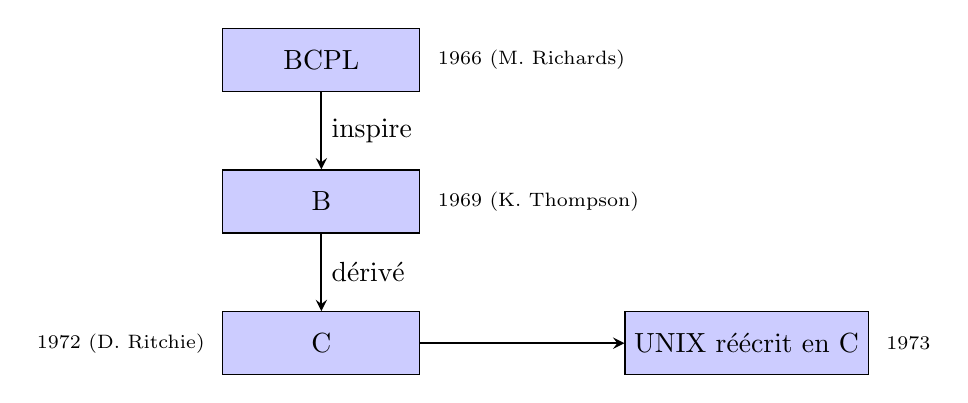
\begin{tikzpicture}[scale=0.9,
    box/.style={rectangle,draw,fill=blue!20,minimum width=2.5cm,minimum height=0.8cm,align=center},
    arrow/.style={->,>=stealth,thick}]

% Timeline verticale
\node[box] (bcpl) at (0,0) {BCPL};
\node[right=0.1cm of bcpl,font=\scriptsize] {1966 (M. Richards)};

\node[box] (b) at (0,-2) {B};
\node[right=0.1cm of b,font=\scriptsize] {1969 (K. Thompson)};

\node[box] (c) at (0,-4) {C};
\node[left=0.1cm of c,font=\scriptsize] {1972 (D. Ritchie)};

\node[box] (unix) at (6,-4) {UNIX réécrit en C};
\node[right=0.1cm of unix,font=\scriptsize] {1973};

\draw[arrow] (bcpl) -- (b) node[midway,right] {inspire};
\draw[arrow] (b) -- (c) node[midway,right] {dérivé};
\draw[arrow] (c) -- (unix);

\end{tikzpicture}
\end{center}

Le C est directement dérivé du langage B (Ken Thompson, 1969), lui-même inspiré de BCPL (Basic Combined Programming Language, Martin Richards, 1966).

\subsection{Versions Majeures}

\begin{definitionbox}{K\&R C (1978)}
Première définition du langage dans "The C Programming Language" par Brian Kernighan et Dennis Ritchie. Standard de facto sans normalisation formelle.
\end{definitionbox}

\begin{definitionbox}{ANSI C / C89 (1989)}
Première standardisation par l'ANSI (American National Standards Institute). Ajout de prototypes de fonctions, qualificateurs \texttt{const} et \texttt{volatile}, bibliothèque standard.
\end{definitionbox}

\begin{definitionbox}{C99 (1999)}
Types \texttt{long long}, \texttt{\_Bool}, nombres complexes. Commentaires \texttt{//}. Déclarations mixtes code/variables. Tableaux de longueur variable (VLA). Fonctions \texttt{inline}.
\end{definitionbox}

\begin{definitionbox}{C11 (2011)}
Support multithreading natif (\texttt{<threads.h>}), assertions statiques (\texttt{\_Static\_assert}), types atomiques (\texttt{<stdatomic.h>}), amélioration Unicode.
\end{definitionbox}

\begin{definitionbox}{C17 (2018)}
Corrections techniques, pas de nouvelles fonctionnalités majeures.
\end{definitionbox}

\begin{definitionbox}{C23 (2023)}
Dernière version. Ajout de \texttt{typeof}, attributs standards (\texttt{[[nodiscard]]}), \texttt{\_BitInt(N)} pour entiers de largeur arbitraire, amélioration des préprocesseur.
\end{definitionbox}

\begin{center}
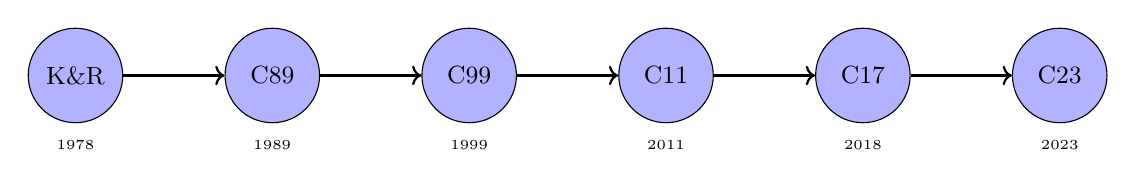
\begin{tikzpicture}[scale=1,
    ver/.style={circle,draw,fill=blue!30,minimum size=1.2cm,font=\small,align=center}]

\node[ver] (k) at (0,0) {K\&R};
\node[below=0.1cm of k,font=\tiny] {1978};

\node[ver] (c89) at (2.5,0) {C89};
\node[below=0.1cm of c89,font=\tiny] {1989};

\node[ver] (c99) at (5,0) {C99};
\node[below=0.1cm of c99,font=\tiny] {1999};

\node[ver] (c11) at (7.5,0) {C11};
\node[below=0.1cm of c11,font=\tiny] {2011};

\node[ver] (c17) at (10,0) {C17};
\node[below=0.1cm of c17,font=\tiny] {2018};

\node[ver] (c23) at (12.5,0) {C23};
\node[below=0.1cm of c23,font=\tiny] {2023};

\draw[->,thick] (k) -- (c89);
\draw[->,thick] (c89) -- (c99);
\draw[->,thick] (c99) -- (c11);
\draw[->,thick] (c11) -- (c17);
\draw[->,thick] (c17) -- (c23);

\end{tikzpicture}
\end{center}

\subsection{Influence et Philosophie}

\begin{examplebox}{Influence du C}
Le C a directement influencé C++, Objective-C, C\#, Java, JavaScript, Go, et Rust. La syntaxe du C (accolades, opérateurs, structures de contrôle) est devenue le standard de facto pour les langages impératifs.
\end{examplebox}

\begin{techbox}{Philosophie de design}
\textbf{Principes fondamentaux:}
\begin{itemize}
\item Confiance au programmeur
\item Pas de vérifications inutiles au runtime
\item Correspondance proche avec le matériel
\item Langage minimal avec bibliothèque standard riche
\end{itemize}

Ces choix expliquent la performance du C mais aussi ses pièges (UB, gestion manuelle de la mémoire).
\end{techbox}

\section{Structure du Cours}

Le cours est organisé en 6 grandes parties couvrant 13 chapitres obligatoires:

\begin{center}
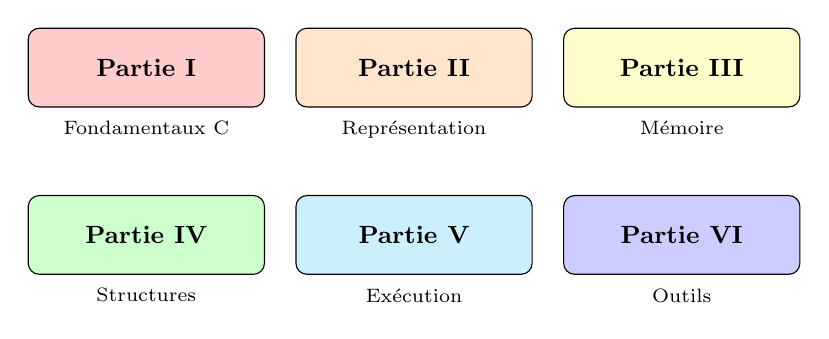
\begin{tikzpicture}[scale=0.85,
    partie/.style={rectangle,rounded corners,draw,fill=blue!20,minimum width=3cm,minimum height=1cm,align=center,font=\small\bfseries},
    node distance=0.5cm]

\node[partie,fill=red!20] (p1) at (0,0) {Partie I};
\node[below=0.05cm of p1,font=\scriptsize] {Fondamentaux C};

\node[partie,fill=orange!20] (p2) at (4,0) {Partie II};
\node[below=0.05cm of p2,font=\scriptsize] {Représentation};

\node[partie,fill=yellow!20] (p3) at (8,0) {Partie III};
\node[below=0.05cm of p3,font=\scriptsize] {Mémoire};

\node[partie,fill=green!20] (p4) at (0,-2.5) {Partie IV};
\node[below=0.05cm of p4,font=\scriptsize] {Structures};

\node[partie,fill=cyan!20] (p5) at (4,-2.5) {Partie V};
\node[below=0.05cm of p5,font=\scriptsize] {Exécution};

\node[partie,fill=blue!20] (p6) at (8,-2.5) {Partie VI};
\node[below=0.05cm of p6,font=\scriptsize] {Outils};

\end{tikzpicture}
\end{center}

\subsection{Détail des Parties}

\begin{definitionbox}{Partie I: Fondamentaux C}
Maîtrise complète de la syntaxe C (structures de contrôle, types, opérateurs, fonctions, compilation).
\end{definitionbox}

\begin{definitionbox}{Partie II: Représentation}
Représentation numérique (binaire, hexadécimal, virgule flottante IEEE 754).
\end{definitionbox}

\begin{definitionbox}{{Partie III: Mémoire, Pointeurs, Tableaux}}
Organisation mémoire, adressage, pointeurs, tableaux 1D/2D, chaînes de caractères.
\end{definitionbox}

\begin{definitionbox}{Partie IV: Structures et Allocation}
Structures, unions, alignement, allocation dynamique (malloc/free).
\end{definitionbox}

\begin{definitionbox}{Partie V: Exécution et Système}
Stack frames, layout mémoire, hiérarchie cache, fichiers POSIX.
\end{definitionbox}

\begin{definitionbox}{Partie VI: Outils et Techniques}
Makefiles, linking, pointeurs de fonctions, préprocesseur, optimisation.
\end{definitionbox}

\begin{warningbox}{Chapitres optionnels}
Deux chapitres optionnels couvrent le multithreading et les sockets réseau.
\end{warningbox}

\subsection{Objectifs du Cours}

\begin{techbox}{Compétences visées}
\begin{itemize}
\item Comprendre les mécanismes sous-jacents du C (pas seulement la syntaxe)
\item Maîtriser l'organisation mémoire et l'adressage
\item Debugger efficacement (GDB, Valgrind)
\item Optimiser les performances (cache, algorithmes)
\item Développer du code système robuste
\item Utiliser les outils professionnels (Make, Docker)
\end{itemize}
\end{techbox}

\section{Prérequis}

\begin{warningbox}{Connaissances requises}
Les étudiants doivent avoir des connaissances basiques en C:
\begin{itemize}
\item Variables et types de base (int, float, char)
\item Structures de contrôle simples (if, for, while)
\item Fonctions et passage de paramètres
\item Pointeurs simples (déclaration, déréférencement)
\item Compilation basique avec gcc
\end{itemize}

\textbf{Ce cours n'est pas une introduction au C.} Les concepts de base sont supposés acquis.
\end{warningbox}

\section{Environnement de Travail}

Tous les travaux pratiques (TP) utilisent un environnement Docker standardisé. Le TP-1 couvre l'installation et la configuration de cet environnement.

\begin{infobox}{Avantages de Docker}
L'utilisation de Docker garantit un environnement identique pour tous les étudiants, indépendamment du système d'exploitation (Windows, macOS, Linux).
\end{infobox}

\begin{center}
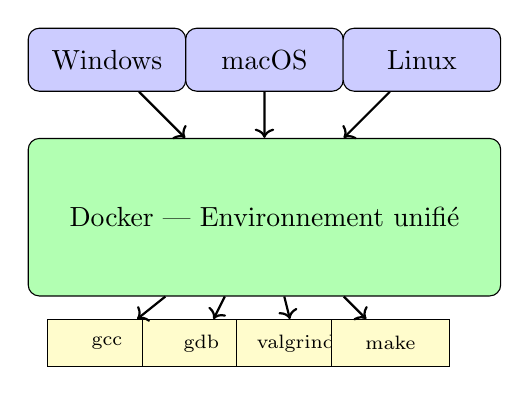
\begin{tikzpicture}[scale=0.8,
    os/.style={rectangle,rounded corners,draw,fill=blue!20,minimum width=2cm,minimum height=0.8cm,align=center},
    docker/.style={rectangle,rounded corners,draw,fill=green!30,minimum width=6cm,minimum height=2cm,align=center},
    tool/.style={rectangle,draw,fill=yellow!20,minimum width=1.5cm,minimum height=0.6cm,align=center,font=\scriptsize}]

\node[os] (win) at (0,0) {Windows};
\node[os] (mac) at (2.5,0) {macOS};
\node[os] (lin) at (5,0) {Linux};

\node[docker] (dock) at (2.5,-2.5) {Docker --- Environnement unifié};

\node[tool] (gcc) at (0,-4.5) {gcc};
\node[tool] (gdb) at (1.5,-4.5) {gdb};
\node[tool] (val) at (3,-4.5) {valgrind};
\node[tool] (make) at (4.5,-4.5) {make};

\draw[->,thick] (win) -- (dock);
\draw[->,thick] (mac) -- (dock);
\draw[->,thick] (lin) -- (dock);

\draw[->,thick] (dock) -- (gcc);
\draw[->,thick] (dock) -- (gdb);
\draw[->,thick] (dock) -- (val);
\draw[->,thick] (dock) -- (make);

\end{tikzpicture}
\end{center}

\begin{techbox}{Contenu de l'image Docker}
L'image Docker (\texttt{elbachirtoure/c-advanced-course:v2.0}) contient:
\begin{itemize}
\item \textbf{Compilateurs:} gcc, g++
\item \textbf{Debuggers:} gdb (avec gdb-dashboard pour meilleure visualisation)
\item \textbf{Outils mémoire:} valgrind, AddressSanitizer
\item \textbf{Éditeurs:} vim, nano
\item \textbf{Outils de build:} make, cmake
\end{itemize}
\end{techbox}

\section{Organisation Pédagogique}

Pour chaque chapitre, le cours comprend trois composantes:

\begin{center}
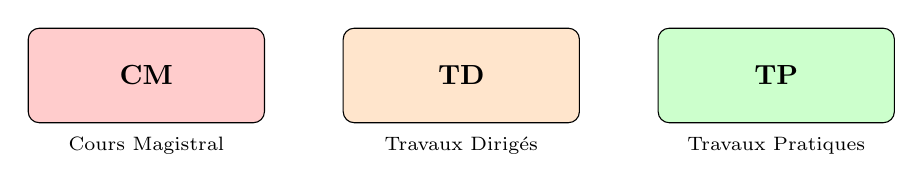
\begin{tikzpicture}[scale=1,
    comp/.style={rectangle,rounded corners,draw,minimum width=3cm,minimum height=1.2cm,align=center}]

\node[comp,fill=red!20] (cm) at (0,0) {\textbf{CM}};
\node[comp,fill=orange!20] (td) at (4,0) {\textbf{TD}};
\node[comp,fill=green!20] (tp) at (8,0) {\textbf{TP}};

\node[below=0.05cm of cm,font=\scriptsize] {Cours Magistral};
\node[below=0.05cm of td,font=\scriptsize] {Travaux Dirigés};
\node[below=0.05cm of tp,font=\scriptsize] {Travaux Pratiques};

\end{tikzpicture}
\end{center}

\begin{definitionbox}{CM (Cours Magistral)}
Présentation des concepts avec visualisations mémoire et exemples techniques.
\end{definitionbox}

\begin{definitionbox}{TD (Travaux Dirigés)}
Exercices d'analyse et de compréhension approfondie des mécanismes. Inclut des exercices forensics d'analyse de dumps hexadécimaux.
\end{definitionbox}

\begin{definitionbox}{TP (Travaux Pratiques)}
Mise en pratique avec compilation, debugging, et implémentation de programmes. Utilisation intensive de GDB et Valgrind.
\end{definitionbox}

\section{Conclusion}

Ce cours vise à former des ingénieurs capables de:
\begin{itemize}
\item Comprendre en profondeur le fonctionnement du C
\item Analyser et optimiser du code système
\item Debugger efficacement des problèmes complexes
\item Développer du code robuste et performant
\end{itemize}


\end{document}
